\chapter{Results and Discussion}
In this section the final model's capabilities are tested and discussed. Previously, the model has been evaluated on labeled data, thus generating a success rate. Below, the model will instead make predictions on unlabeled data, and instead output a confidence in its prediction.

Later on various things about the work are brought up for discussion.

\section{Real and artificial transition regions}

While we up to this point maily have focused on leave-one-out and validation set accuracies we have not in detail studied what the classifier output looks like. We are specifically interested in examining how well performance is when the robot moves across a \emph{transition region}, a region where the surface type changes from grass to nongrass or vice versa. Ideally the prediction should rapidly change according to the new target surface. 

This can be accomplished in two different ways. The first revolves around creating a test set by concatenating the last parts of each session. By doing this, we artificially generate transition region data which we can predict on. Examining these predictions we get a feel for what output the predictor may generate when moving from one surface to the next. The second method is to simply use real-world measurements from when the robot moves across a surface. We should see that at the time point when the robot has reached the transition the prediction change accordingly. 

In the first test, four surfaces are concatenated into a sequence: grass, asphalt, grass, tiles. The predictions are shown in the top part of figure \ref{fig:artificial1}. Below, the predictions are median filtered with filter length $L=5$, see section \ref{surface_change}. The outliers are removed, rendering a very accurate description of the scene. 

Two more challenging surfaces according to table \ref{tab:loo} are soil and gravel. In figure \ref{fig:artificial2} the predictions on artificial transitions including these are displayed. With median filtering we obtain equally good results. Something worth noting in the two figure is that the surface transition is delayed by two steps after the median filtering. It is important to be aware of what distance this corresponds to in the physical world, since we do not want to detect an edge long after it is passed. Each prediction uses 25 samples, and with a delay of two predictions this means a 50 sample delay. With a sample frequency of 200 Hz, this means a 0.25 second delay in the edge detection, or traveling at the speed $v=0.3$ m/s, a delay corresponding to $0.3\cdot0.25=0.075$ m.

Looking at the high leave-one-out accuracies in table \ref{tab:loo}, the results of classifications upon the artificial transitions may not come as a surprise, as they are based on the same data. What we can see here, however, is that not only does the model classify correctly, but it does so with a very high confidence. To test the model even further, it will make predictions of real world transitions, not included in our dataset. Figure \ref{fig:trans_tgtg} shows a transition from grass to tiles, and figure \ref{fig:trans_gg} a transition from grass to gravel. Focusing on the median filtered predictions, we see that outside the transition region, the model works well for classifying both materials. What happens around the transition is perhaps more interesting. In the previous figures, the predictions went from 1 to 0 and vice versa in just one step. Here, it takes a while before the model reaches zero-outputs. There are two possible explanations for this. First of all, in the artificial transitions, the surface went from a perfect grass surface to a perfect non-grass surface at an instance. In real transitions, there might be some overlap of grass on the non-grass surface, making the model unsure of what it sees. Another explanation could be that one sensor is facing straight down, whereas the other one looks slightly more forward. Hence, the model is perceiving both grass and tiles simultaneously during a short time. 

The results show great promise, but the work is still at an early stage. The surfaces in the four transitions were intentionally free from as many obstructions as possible. When facing surfaces with characteristics not taken into regard by the model, the results will not likely be as good. 

\begin{figure}
	\centering
	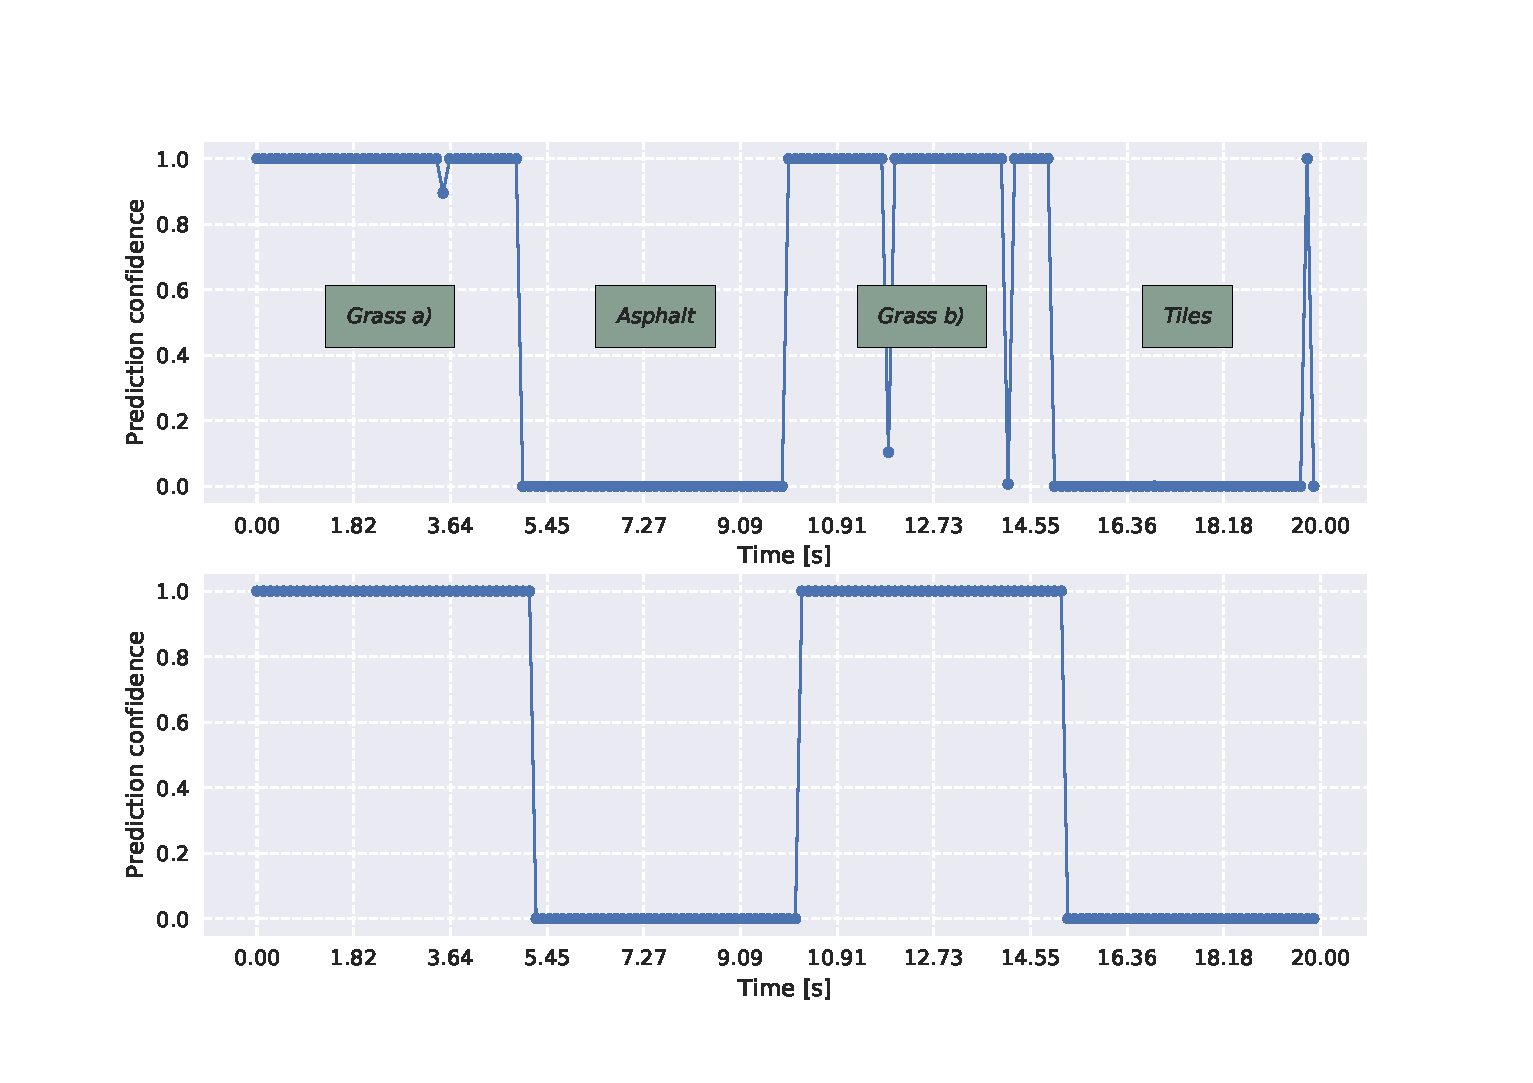
\includegraphics[scale=0.5]{figs_temp/varmats1}
	\caption{Predictions on an artificial transition region created using samples from four different regions. The bottom figure shows the median filtered predictions with filter length $L=5$.}
	\label{fig:artificial1}
\end{figure}

\begin{figure}
	\centering
	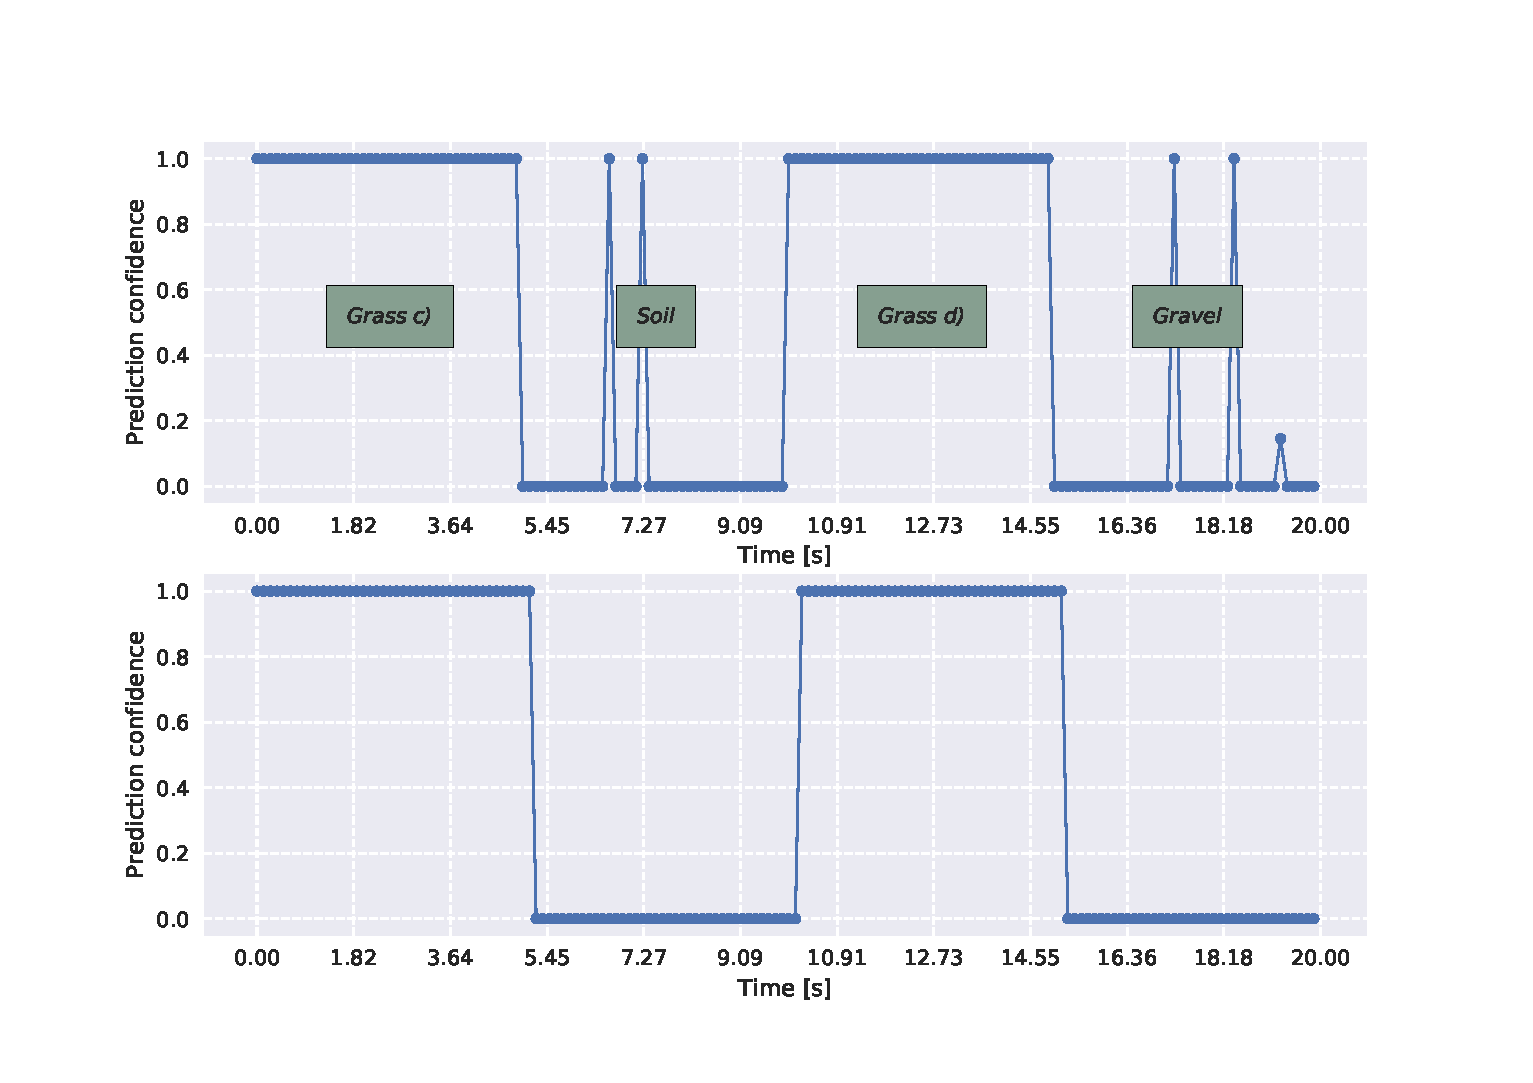
\includegraphics[scale=0.5]{figs_temp/varmats2}
	\caption{Predictions on an artificial transition region created using samples from four different regions.}
	\label{fig:artificial2}
\end{figure}

\begin{figure}
	\centering
	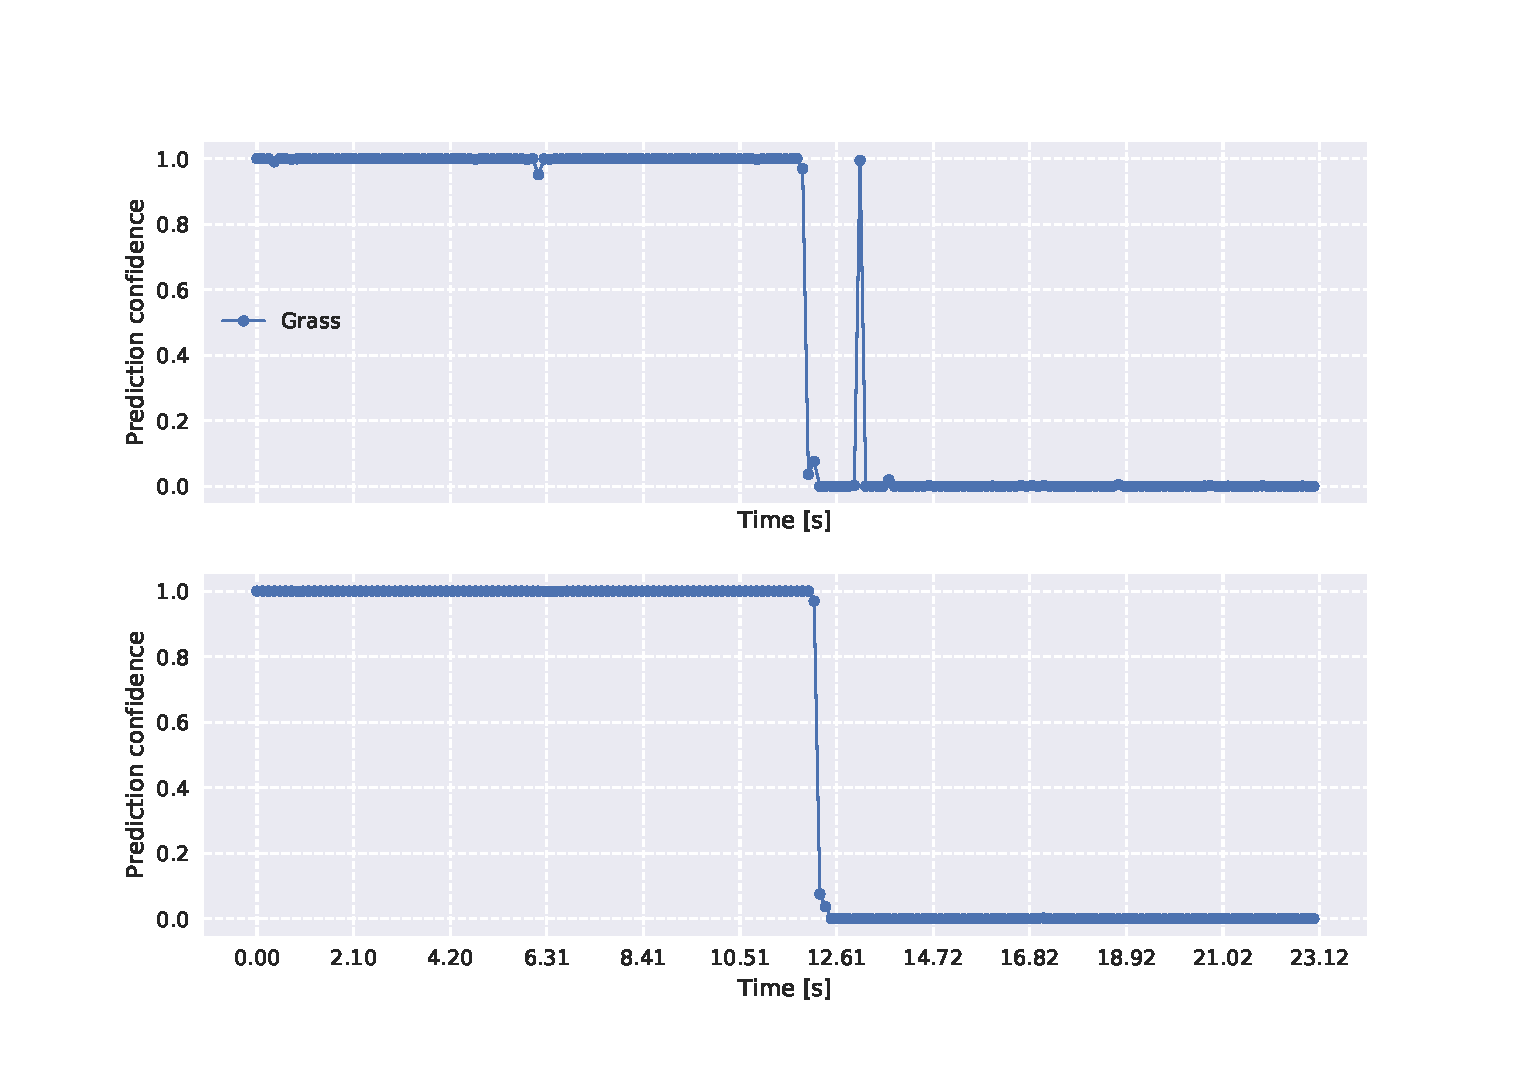
\includegraphics[scale=0.5]{figs_temp/transition_grass_tiles_grass}
	\caption{Predictions from a real-world test where the robot moved from grass to a tiled pavement.} 
	\label{fig:trans_tgtg}
\end{figure}

\begin{figure}
	\centering
	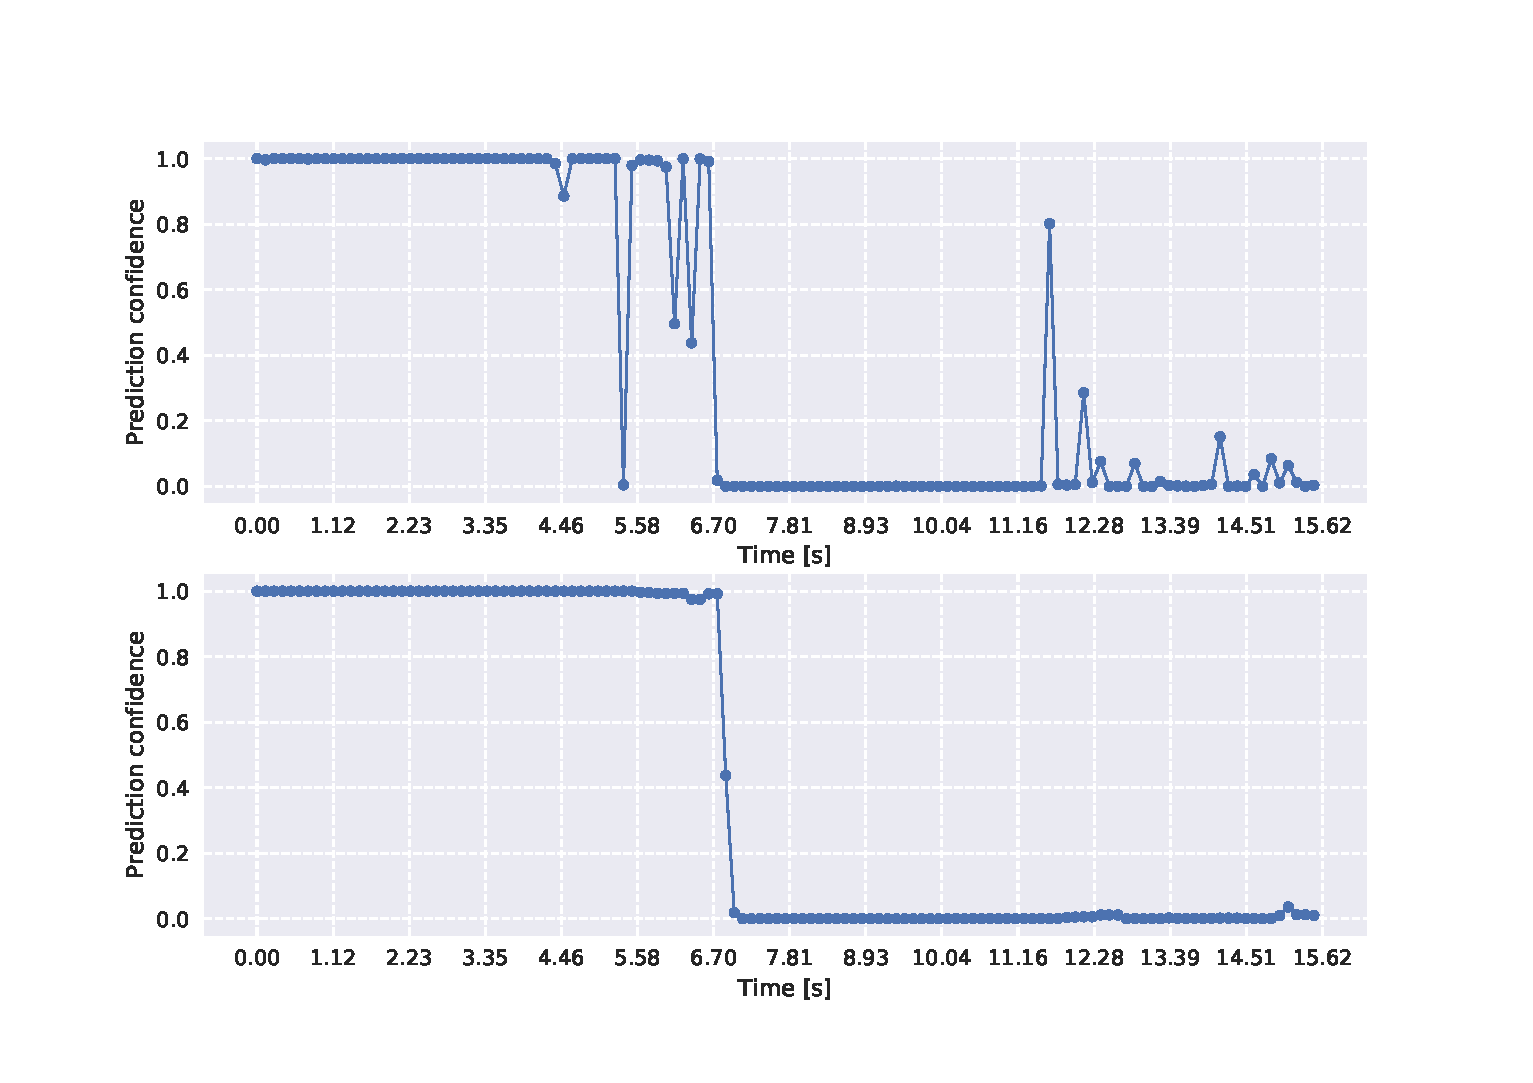
\includegraphics[scale=0.5]{figs_temp/transition_grass_gravel2}
	\caption{Predictions from a real-world test where the robot moved from grass to gravel.}
	\label{fig:trans_gg}
\end{figure}

\section{Difficult surfaces}
While we only have five material classes in this work, each class can be broken down to multiple subclasses. Taking grass as an example, it may vary in a wide range of attributes such as length, humidity and sparsity to name a few. Therefore it is important to gather a dataset as diverse as possible, so that the model has trained on all common varieties of each surface. 

However, the model can only be prepared for so much, and an often critical aspect of any machine learning system is its performance on dissimilar data. It is difficult to foresee how a complex neural network will interpret a surface displaying characteristics not included in training. For instance, what would the model make of a lawn which is partially covered by leaves and twigs; or a surface type it has never seen before? Perfecting the model to work in any surrounding calls for a good sense of what difficulties may occur, as well as a large time investment. 

%\section{Moisture}

%One particularly challenging aspect of adequately classifying surfaces is the ever-changing environmental conditions surronding the sensor. Of particular interest is the moisture content in the surfaces of interest. Greater soil moisture implies higher dielectric constant, which in turn increases radar wave scattering \citep{rappaport_2006}. Thus a single surface may very well change its scattering properties over time. 

% More things that make selecting data tricky

%\section{Surface variances}


%Such effects is difficult to account for when selecting data. Gather a dataset as diverse as possible



\section{Feature Extraction and Model Selection}
Table \ref{tab:loo} is in many ways a very telling one. Here, each sample session was classified without using any of the samples from the session at hand. Instead, all other sessions were used in training. Six different methods of classification were evaluated; two linear and four nonlinear. 

First and foremost it is noted that each tested method performed at the very least \emph{decently}. One may argue that the \gls{lstm} model is unstable or that using \gls{lda} produces lower accuracy predictions, but they nonetheless generated accuracies above 97\% on average. Considering these are the lower-performing classifiers, and the remaining ones perform even better, suggests that the performed feature extraction captures, or at least maintains, the cruicial information in the original data. 

Some may argue that no feature extraction should be performed when working with deep neural networks; that the networks are complex enough to find good features on their own. If this is true, the network may yield a better result by omitting the feature extraction as this could discard information in the original data. However, since much of the informations seems to be found in how signals evolve over time, a network with no feature extraction would require multiple sweeps to be concatenated into one feature vector in order to be able to find these time dependencies. Say it would take 25 (downsampled) sweeps, each with 14 range bins. Each sweep would then produce 28 features as the real and imaginary part are divided into separate features. The feature vector to such a network would then consist of $25\cdot 28=700$ features. While this could \textit{potentially} slightly increase the already great accuracies, the feature extraction reduces the number of features (and thereby computational cost) and - if done properly - represents samples with more robust features that are material specific.

On a different note, the final choice of classifier is also debatable. The \gls{dnn} classifier was chosen mainly because of its high leave-one-out scores in table \ref{tab:loo}. But without blindly chasing an accuracy as high as possible, the results of the linear models are good enough to suggest that the data could be at least \textit{approximately} linearly separable. If it were, a non-linear model would not be necessary, hence further investigation in linear models is motivated.

\section{Errors and Uncertainties}
As with all works, there are things that can go wrong due to either technical reasons or human reliability. The data collecting process is a prime example of where human reliability is inevitable. Here, fundamental decisions are made, which the entire work is based upon. For instance, in general, one strives for a dataset where the numbers of samples from each class are as balanced as possible. But the question of what a balanced dataset \textit{is}, sometimes holds multiple answers. In this work, there are four different types of materials belonging to class 0 (not grass) and one belonging to class 1. A natural question to ask oneself is whether there should be equally many samples for each \textit{material}, or equally many for each \textit{class}. We have chosen to balance the dataset so that there are approximately as many samples in each class. If all grass surfaces looked the same, this would perhaps make the model biased in its predictions, but due to the great variety among grass surfaces the bias is eliminated.

Another risk when collecting data is obtaining too little of it. However, looking at how high accuracies the models achieve as well as how little improvement the data augmentation yields, it is not likely that we provide too little data to our models.

A more technical uncertainty regards the assumption of a constant velocity. When facing a rough terrain or steep hills, the robot's velocity is bound to change. As both the \gls{dft} and autocovariance require a consistency in the spacing between sample points, we cannot tolerate too large variations in velocity. Hence, to sample at regular distaces the sampling could be controlled by positional feedback from the robot rather than a fixed sampling frequency.

While this work has not put much focus on \textit{live} classifications, this does pose a new limitation on the model. Ideally we want the system to collect $T$ samples, and make an instantaneous prediction so that $T$ new samples can be collected right away. By running the system on a single thread, however, the time it takes to generate a prediction delays the data collecting process with some time $t_{cl}$, as only one process can be ran at a time. An alternative could be to handle the classifications in a separate thread. That way, data could be collected continously, while classifications are performed in parallel. Doing this requires caution. If the time it takes to generate a classification exceeds the time it takes to collect $T$ samples, i.e. $t_{cl}>T/F_s$, a delay will accumulate over time. After a while predictions would be irrelevant as they would be based on surfaces far behind the robot. A natural limitation to assign the model is therefore
\begin{equation}
	t_{cl} \le \frac{T}{F_s}.
\end{equation}
The time $t_{cl}$ has not been discussed in this work, but is highly relevant to study in the future.



% This remarkable result means that given a random sample from the dataset collected, with no samples from the session the sample was taken from used in training, we can correcly classify the surface as grass or non-grass 39/40 times even with the lower-performing classifiers. With the top performing fully connected model, even higher accuracy was obtained with a low standard deviation. 


